\documentclass{article}
\usepackage[left=2.5cm,right=2.5cm, top = 2.5cm, bottom = 3cm]{geometry}
\usepackage{graphicx}
\usepackage{natbib}
\usepackage{hyperref}
\usepackage{todonotes}
\usepackage{booktabs}
\usepackage{amssymb}
\usepackage{amsmath}

\newcommand{\sd}{s}
\newcommand{\mean}{\bar{y}}


\begin{document}
% \SweaveOpts{concordance=TRUE}

% \title{A bootstrap-based comparison of ILI intensity thresholds from the moving epidemic and WHO methods}
\title{An empirical assessment of influenza intensity thresholds obtained from the moving epidemic and WHO methods}
% \author{Johannes Bracher$^{1, 2}$, Jonas Littek$^1$}
% \date{ \small
% $^1$Karlsruhe Institute of Technology (KIT), Chair of Statistics and Econometrics\\
% $^2$Heidelberg Institute for Theoretical Studies (HITS), Computational Statistics Group}

\maketitle

\abstract{The moving epidemic method (MEM) and the WHO method are widely used to determine intensity levels for seasonal influenza. The two approaches are conceptually similar, but differ in two aspects. Firstly, the MEM involves a log transformation of incidence data, while the WHO method operates on the original scale. Secondly, the MEM uses more than one observation from each past season to compute thresholds, fixing the total number to include. The WHO method uses only the highest value from each season. To assess the impact of these choices on thresholds and exceedance proportions we perform simulation studies which are based on re-sampling of ILI data from France, Spain, Switzerland and the US. When no transformation is applied, a large proportion of season peaks are classified as high or very high intensity. This can be mitigated by a logarithmic transformation. When fixing the total number of included past observations, thresholds increase the more seasons are available. When only few are available, there is a high chance of classifying a new season peak as high or very high intensity. We therefore suggest using one observation per season and a log transformation, i.e.\ a hybrid of the default settings of the MEM and WHO methods.}

% \medskip

% \noindent \textbf{Keywords:} influenza-like illness, intensity thresholds, moving epidemic method, seasonal influenza, WHO method

\section{Introduction}

Following the 2009 influenza H1N1 pandemic, the need for a rapid assessment tool for influenza intensity was recognized. The \textit{Review Committee on the Functioning of the
International Health Regulations and on Pandemic Influenza (H1N1)} recommended that member states perform yearly updates and evaluations of intensity thresholds \citep[p.118]{WHO2011}. In the subsequent \textit{WHO Pandemic Infuenza Severity Assessment (PISA)} guideline \citep{WHO2017} the so-called WHO method \citep{WHO2014} and the moving epidemic method (MEM; \citealt{Vega2013, Vega2015}) were recommended to this end. The latter, which is also employed by the European Centre for Disease Prevention and Control (e.g., \citealt{ECDC2017}), has been adopted by numerous national public health agencies (e.g., \citealt{Dahlgren2019}, \citealt{Rakocevic2019}, \citealt{RedondoBravo2020}, \citealt{Vos2019}); see Supplement C for an overview of recent applications. The statistical properties of the MEM and WHO methods, however, have not yet been studied in detail. We here address this aspect via simulation experiments based on re-sampling of historical influenza data. Our results indicate that it may be beneficial to use a hybrid of the default settings of these two methods.% These are complement with some analytical statistical results.

% The article is structured as follows. Section \ref{sec:definitions} provides concise definitions of the MEM and WHO methods, highlighting two differences between these conceptually similar approaches. Section \ref{sec:recent_applications} consists of an overview of published applications of the MEM and WHO methods. This is followed by a brief examination of statistical properties of the two methods in Section \ref{sec:analytical}. In Section \ref{sec:simulation} we describe our simulation approach and the results based on historical data from France, Spain, Switzerland and the United States. Section \ref{sec:discussion} concludes with a discussion.

\section{Definition of the moving epidemic and WHO methods}
\label{sec:definitions}

We describe the computation of influenza/influenza-like illness (ILI) intensity thresholds, framing the MEM and WHO methods as two special cases of the same general approach. We assume that thresholds are based on weekly data (typically incidences) from $m$ past seasons and applied to the ($m + 1$)-th season. \cite{Vega2015} recommend to use $5 \leq m \leq 10$ seasons for the MEM to ensure a recent data basis. Computation of thresholds then proceeds as follows:

\begin{enumerate}
\item Select the $n$ largest observations from each of the $m$ past seasons to construct a set of reference observations.
\item Apply an (invertible) transformation to all selected observations.
\item Assume that the $m \times n$ transformed reference observations come from a normal distribution and compute estimates $\mean, \sd$ of its mean and standard deviation.
\item Define intensity thresholds on the transformed scale as quantiles of the normal distribution N$(\mean, \sd^2)$. A common choice for both methods is
\begin{itemize}
\item the 40th percentile $\mean - 0.25 \sd$ as the threshold between low and medium intensity;
\item the 90th percentile $\mean + 1.28 \sd$ as the threshold between medium and high intensity;
\item the 97.5th percentile $\mean + 1.96\sd$ as the threshold between high and very high intensity.
\end{itemize}
\item Transform thresholds back to the original scale (e.g. using the exponential function if a log trnsformation was used).
\end{enumerate}

\noindent The MEM and WHO methods are special cases of this procedure:
\begin{itemize}
\item In the WHO method, $n = 1$ observation per season is used and by default no transformation is applied. If peak incidences vary strongly across seasons, a log transformation is recommended \citep{WHO2017}. 
\item In the MEM method, the default transformation is the natural logarithm, while the number of included observations per season is set to $n = 30/m$, rounded to the nearest integer. The total number of historical observations is thus kept approximately fixed.
\end{itemize}
The rationale behind the percentile-based approach is that ``about 50--60\% of the season peaks should be above the moderate threshold, $\pm 10\%$ above the high threshold and $\pm 2.5\%$ above the extraordinary threshold'' \citep{WHO2017}.

The implementation of the moving epidemic method in the R package \texttt{mem} \citep{Lozano2020} permits the user to choose $n$, $m$, and $f$ (\texttt{i.type.intensity	= 5} for no transformation, \texttt{i.type.intensity = 6} for the log transformation). The term \textit{moving epidemic method} could thus also be used as an umbrella term for the general procedure described above. We here use it in a more narrow sense for the specification from \cite{Vega2015}, reflected in the default settings of the \texttt{mem} package.

In previous works (\citealt{WHO2014, Vega2015}), the above thresholds have been described as upper ends of one-sided confidence intervals for the the arithmetic (WHO method) or geometric mean (MEM) of the reference observations. This, however, is imprecise terminology as in the computations the standard deviation $\sd$ rather than the standard error $\sd/\sqrt{nm}$ is used (see documentation of the \texttt{mem} package and \citealt{WHO2014}, p. 69). We note that the use of actual confidence intervals is also possible in the \texttt{mem} package (\texttt{i.type.intensity = 1} for the geometric, \texttt{i.type.intensity = 2} for the arithmetic mean). However, thresholds for all levels will then converge to the arithmetic or geometric mean if sufficient historical data are available. As illustrated in Supplement B, this is not a desirable behaviour.
 

\section{Simulaton study}
\label{sec:simulation}

\subsection{Goal}

We aim to assess how thresholds depend on the employed transformation, the number of observations $n$ used per season and the number $m$ of seasons included. In particular, the following aspects are of interest:

\begin{itemize}
\item The application of a logarithmic transformation is expected to lead to higher thresholds for the extreme categories and thus a lower proportion of seasons peaks classified as high or very high.
\item In the MEM, the reference set also contains past obervations which are not actually peak observations. This may introduce a downward bias in thresholds, especially if due to a small number $m$ of available seasons $n$ is large.
\end{itemize}
The latter aspect is intuitive, but also supported by formal statistical considerations detailed in Supplement A. These imply that thresholds are unbiased for $n = 1$ in the sense that, as intended, they will be exceeded by around 40\%/90\%/97.5\% of the season peaks in the long run. When $n > 1$, thresholds will tend to be lower and exceeded more frequently.

\subsection{Simulation setup}
\label{subsec:simulation_setup}

We compare four versions of the general approach described in Section \ref{sec:definitions}:
\begin{enumerate}
\item[(a)] No transformation, $n = 1$. This corresponds to the WHO method.
\item[(b)] No transformation, $n = 30/m$.
\item[(c)] Logarithmic transformation, $n = 1$.
\item[(d)] Logarithmic transformation, $n = 30/m$. This corresponds to the MEM approach.
\end{enumerate}
In order to closely mimic the seasonal patterns of influenza, we re-sample historical surveillance data rather than generating fully synthetic data. Assume we have $M$ years of historical data on a measure of influenza activity. We then repeat the following steps 500 times:

\begin{itemize}
\item Sample a sequence of 15 seasons from the $M$ available seasons. This is done with equal probability for each season and \textit{with replacement}, meaning that the same season can appear more than once. This approach is called the \textit{seasonal block bootstrap} \citep{Politis2001}.
\item For each value $m = 5, \dots, 15$:
\begin{itemize}
\item Restrict the generated sequence to the first $m$ seasons.
\item Apply approaches (a)--(d) to compute thresholds for medium (40th percentile), high (90th percentile) and very high intensity (97.5th percentile).
\item Compute which fraction of all $M$ available historical season peaks would be classified as low, moderate, high and very high.
\end{itemize}
\end{itemize}
The range $m =5, \dots, 15$ is motivated by the range of values found in real-world applications, see our overview in Supplement C. All analyses were performed using the R language for statistical computing \citep{RCT2020} and the package \texttt{mem} \citep{Lozano2020}.

\subsection{Data}

We use publicly available influenza surveillance data from four countries. Data on the weekly incidence of influenza-like illness in France, 1985--2019, were obtained from Réseau Sentinelles (INSERM/Sorbonne Université, \url{https://www.sentiweb.fr}, \citealt{Flahault2006}). Data on weekly confirmed influenza cases in Spain, 1998--2019, were extracted from graphs shown in the \textit{Informe Anual} of the \textit{Sistema de la vigilancia de gripe en Espa\~na} (\url{https://vgripe.isciii.es/}; \citealt{SVGE2019}). Weekly ILI counts from Switzerland, 2000--2016, collected by the Swiss Federal Office of Public Health are available in the R package \texttt{HIDDA.forecasting} \citep{Held2019}. Weekly weighted ILI (wILI) data at the US national level from CDC FluView \citep{Charbonneau2019}, 1998--2017, were obtained via the CDC FluSight influenza forecasting platform (\url{https://github.com/FluSightNetwork/cdc-flusight-ensemble/}). These wILI values correspond to the fraction of general practitioner visits due to influenza-like symptoms. All four time series are displayed in Figure \ref{fig:data}, with the pandemic 2009/2010 season removed. We also show boxplots of the first through sixth largest observation per season. Not surprisingly, values on average get smaller for increasing ranks. Interestingly, they also get less dispersed, meaning that variability among e.g.\ the sixth largest observations per season is smaller than among the peak values. 

% mention exact definition, source, number of seasons

\begin{figure}[h]
\center
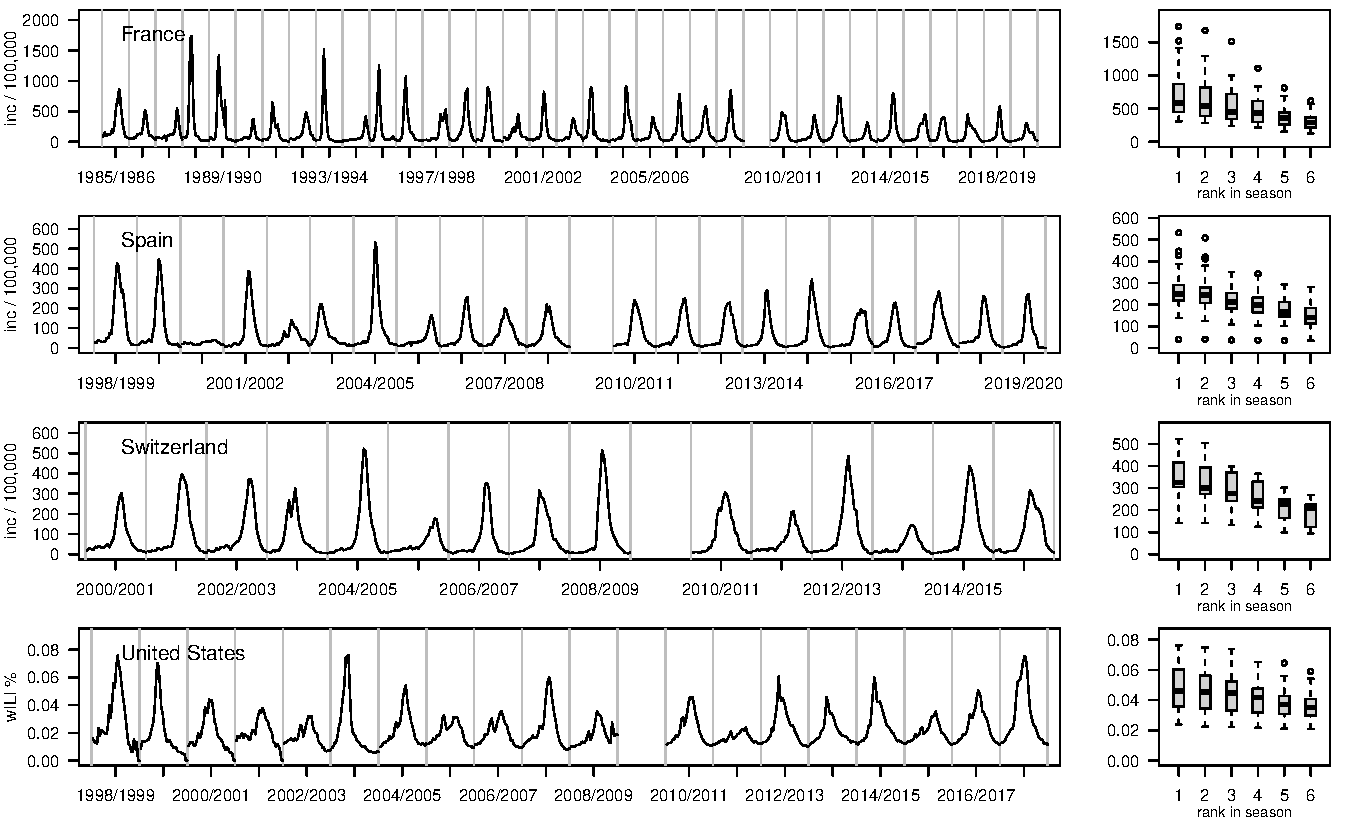
\includegraphics[width=0.9\textwidth]{figure/plot_data.pdf}
\caption{Time series of influenza activity measures in four countries: Weekly ILI cases per 100,000 population in France, 1985--2019; weekly number of confirmed influenza cases per 100,000 population in Spain, 1998--2019; weekly ILI cases per 100,000 in Switzerland, 2000--2016; weekly wILI values in the United States, 1998--2017. Off-season weeks are omitted in the plot, with grey lines delimiting the different seasons. The right column shows boxplots of the largest value per season, second largest etc.}
\label{fig:data}
\end{figure}


\subsection{Results}

Results from our simulation study are shown in Figures \ref{fig:results1} (France, Spain) and \ref{fig:results2} (Switzerland and US). In the first and third colum of each figure we also show an analytical approximation of the expected thresholds, see Supplement A for details. In all four countries, using a log transformation leads to increased thresholds, in particular for the high and very high levels. Especially in France and Spain, thresholds obtained without the log transformation are too low, as can be seen from the large proportion of season peaks classified as very high (around 10\% when using $n = 1$). As expected, when letting the number of observations used per season depend on the number of available seasons via $n = 30/m$, average thresholds increase in $m$. As a particularly striking example, the  average threshold for high intensity in France (when using a log transformation) increases from 834 for $m = 5, n = 6$ to 1011 for $m = 10, n = 3$ and 1080 for $m = 15, n = 2$. For $n = 1$, in which case thresholds can be interpreted as unbiased (Supplement A), the average is 1147. Including historical observations which are not from actual peak weeks thus leads to a considerable lowering of alarm thresholds and will increase the number of alerts for high and very high influenza activity. This is not surprising given the pronounced differences between the distribution of season peak values and e.g. fifth largest observation per season, see right column of Figure \ref{fig:data}. In the US and France, on average one in three season peaks is classified as high and one in seven as very high intensity when applying the MEM with log transformation and $m = 5, n = 6$. This is rather far from the intended excedance probabilities of 10\% and 2.5\%.

\begin{figure}
\centering
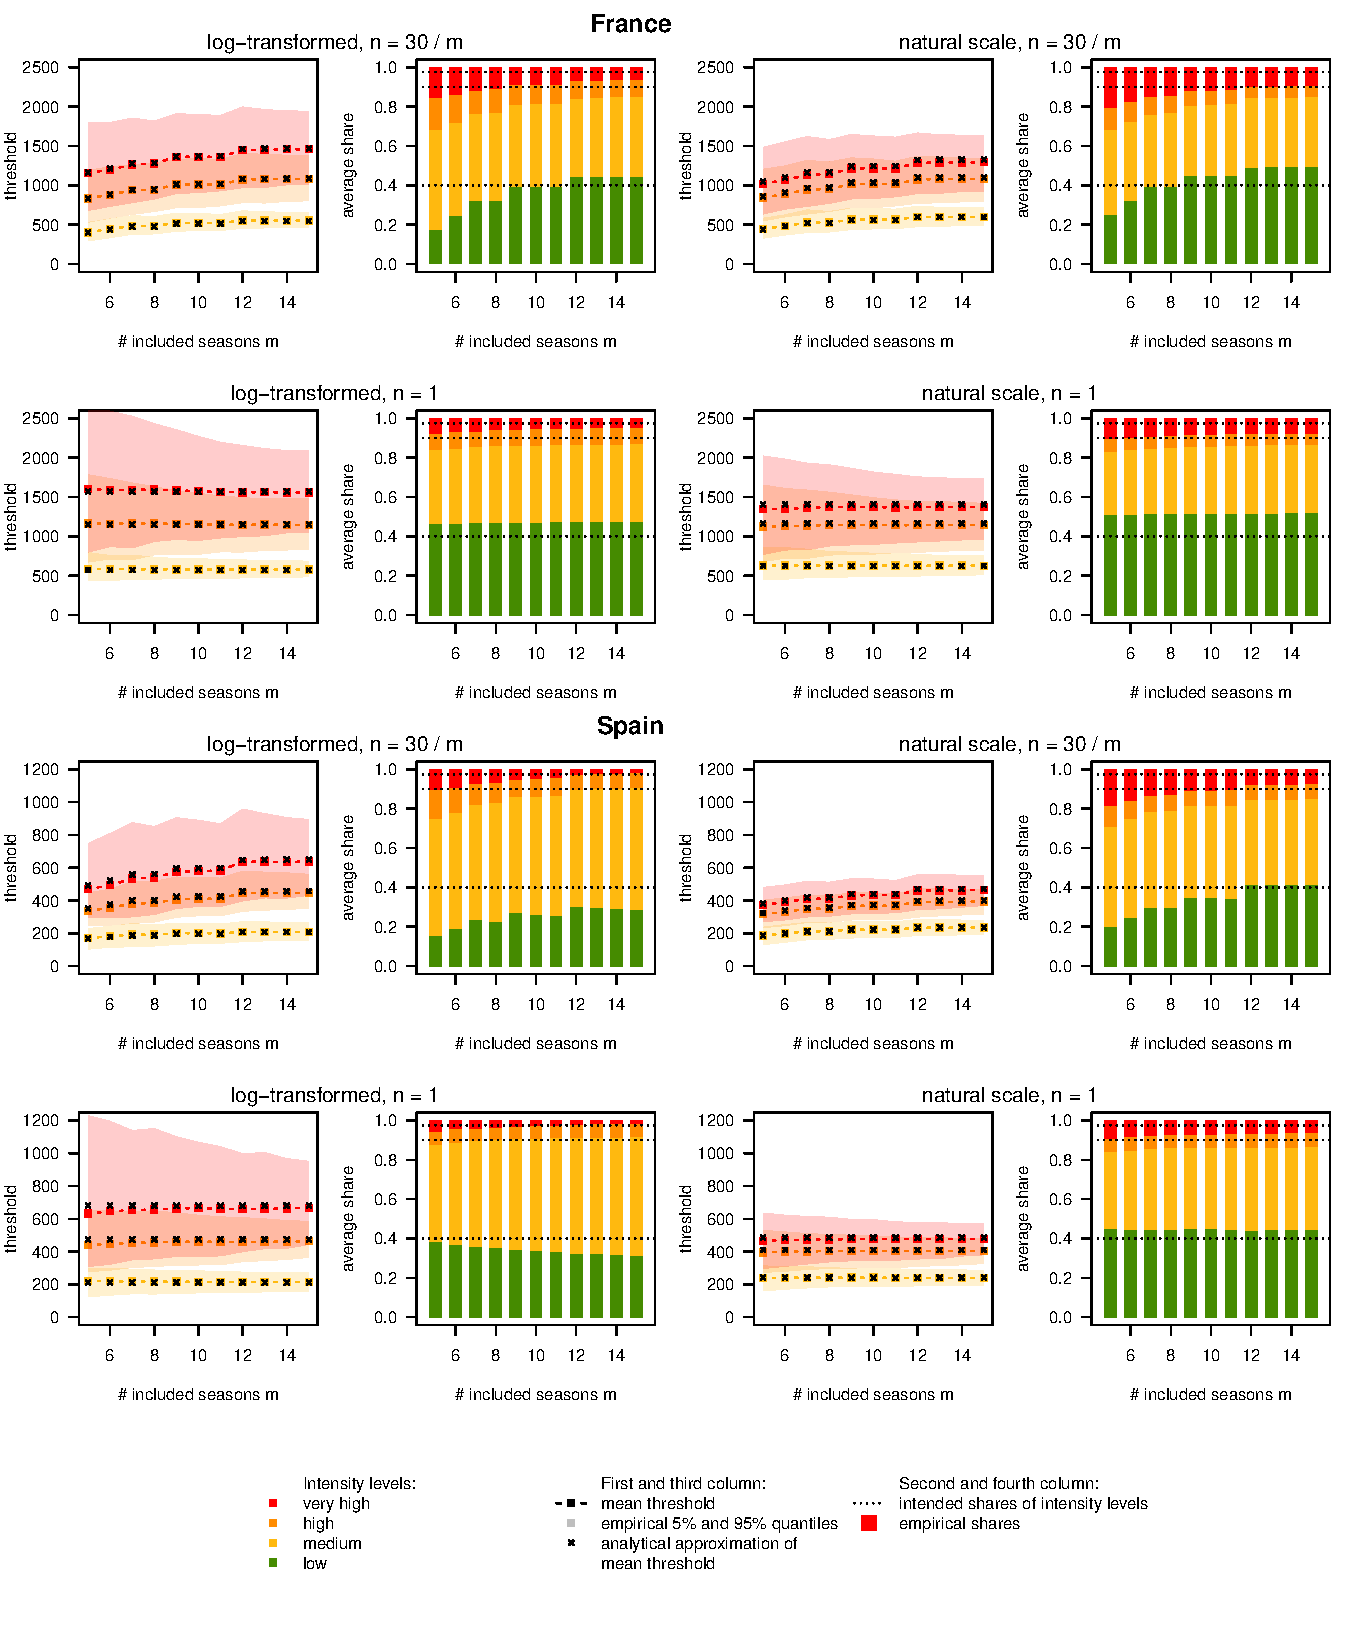
\includegraphics[page=1, width=0.95\textwidth]{figure/plot_results.pdf}
\caption{Results of re-sampling simulation study, France and Spain. First and third column: mean intensity thresholds along with bands delimited by the empirical 5\% and 95\% quantiles. Analytical approximations of the mean threshold values are marked as small black dots. Second and fourth columns: resulting average shares of seasons classified as low, medium, high and very high intensity.}
\label{fig:results1}
\end{figure}

\begin{figure}
\centering
\includegraphics[page=2, width=0.95\textwidth]{figure/plot_results.pdf}
\caption{Results of re-sampling simulation study, Switzerland and United States. First and third column: mean intensity thresholds along with bands delimited by the empirical 5\% and 95\% quantiles. Analytical approximations of the mean threshold values are marked as small black dots. Second and fourth columns: resulting average shares of seasons classified as low, medium, high and very high intensity.}
\label{fig:results2}
\end{figure}

When always using $n = 1$, the average thresholds and shares of the different categories are more well-behaved also for small $m$. This holds especially when applying a log transformation, even though certain mismatches with the nominal exceedance probabilities remain. Also, there is considerable variability in the estimated thresholds (shaded areas in Figures \ref{fig:results1} and \ref{fig:results2}). These difficulties, however, are inherent in the problem of estimating a 90\% or 97.5\% quantile based on 5--10 observations.

% The increase of thresholds obtained with $n = 30/m$ as more historical data accumulate is not only a statistical tendency. For all four countries, the probability that the threshold for high intensity increases when using the first ten rather than only the first five years of a sampled sequence was around 90\%. For illustration of this aspect, consider the following example: We repeat a sequence of five ILI seasons from France (2014--2019) four times to obtain a time series of twenty seasons. We then apply the moving epidemic method with log transformation and $n = 30/m$ using the first $m = 5, 6, \dots, 20$ years of data, mimicking the development of thresholds as more historical data become available. As can be seen from the top panel of Figure \ref{fig:example_france}, this results in gradually increasing thresholds, despite the fact that the data in each five-year block behave the same. For example, season 6 is classified as very high intensity, but seasons 11 and 16 are not, even though they are identical to season 6 and the respective data used to construct thresholds follow exactly the same patterns. The bottom panel shows results obtained for the same time series with $n = 1$. While thresholds fluctuate quite a bit (with fluctuations dampening as the time series gets longer), there is no systematic trend.



%\begin{figure}
%\center
%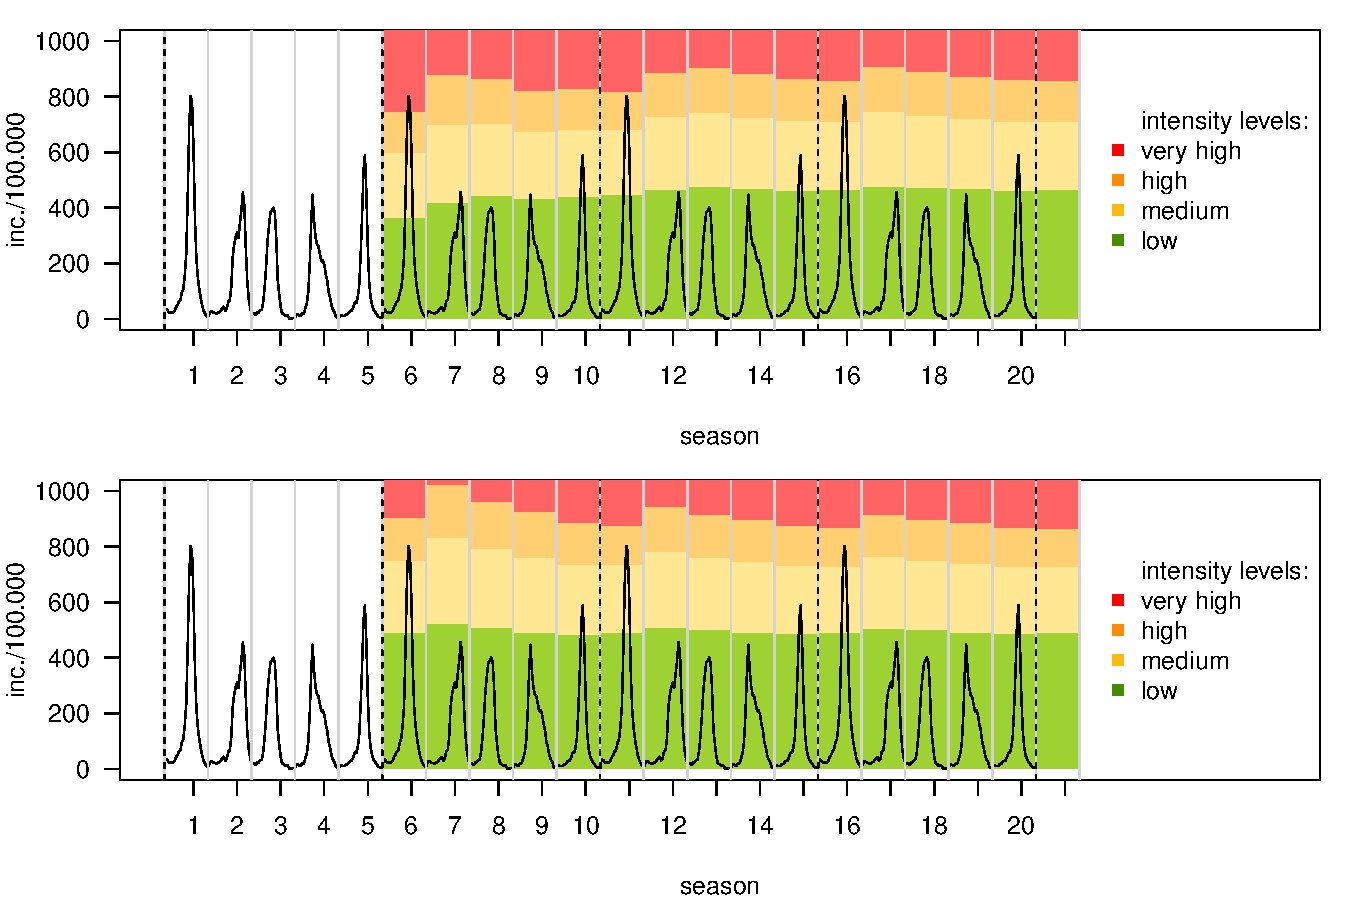
\includegraphics[scale=0.6]{figure/example_france.pdf}
%\caption{Toy example to illustrate increasing thresholds as historical data accumulates: Data from France, 2014/2015--2018/2019 are appended three times and thresholds are computed using $m = 5, \dots, 15$ years of training data. The thresholds based on years 1 through $m$ are overlaid with the incidence time series from the $(m + 1)$-th year.}
%\label{fig:example_france}
%\end{figure}



\section{Discussion}
\label{sec:discussion}

We provided a statistical assessment of implementation choices in a widely used framework for the computation of influenza intensity thresholds. We found that applying a log transformation led to better behaved thresholds and closer to nominal exceedance rates. Concerning the question of how many observations per historical season should be included to computate thresholds, we found that the common choice $n = 30/m$ results in too low thresholds when few historical seasons are available. We therefore recommend adopting $n = 1$ irrespective of the number of available historical seasons. This is possible in the available \texttt{R} package \texttt{mem} by setting \texttt{i.n.max = 1} when the function \texttt{memmodel} is called.

% We focused on the computation of influenza intensity thresholds, but the same general arguments apply to the computation of thresholds to determine the onset of a season \citep{Vega2012}. As variability among observations around the season onset may be lower than around the peak the problem may be less severe; we did not assess this empirically as not all our data sets fully covered the off-season.

We think that a simple and interpretable tool with a well-documented and open source software implementation like \texttt{mem} is a valuable tool in practice. The use of a standard approach at the European level will improve comparability of results, facilitating the evaluation and refinement of the tool. With this work we hope to contribute a statistical perspective on this topic which complements public health practitioners' experience from applied analyses.


\section*{Data and code}

Materials to reproduce the presented results are available at \url{https://github.com/jbracher/mem}.

\section*{Author contributions}

Study concept: JB; Data processing: JB and JL; Literature review: JB and JL; Statistical analysis / implementation: JB; Writing and editing: JB and JL.


\section*{Acknowledgements}

We would like to thank Laura Werlen for helpful feedback. Johannes Bracher was supported by the Helmholtz Foundation via the SIMCARD Information and Data Science Pilot Project.

\bibliographystyle{apalike}
\bibliography{bibliography_mem}
\end{document}